\chapter{Zadanie projektowe}

Zadaniem projektowym tej części naszej pracy było przygotowanie oraz dobranie optymalnych nastawów regulatorów w środowisku Matlab. W części a) należało dobrać strukturę i nastawy dwupętlowego układu regulacji PI/PID z odsprzęganiem i bez odsprzęgania. Kolejno, należało zaprojektować i zaimplementować analityczny regulator predykcyjny z uwzględnieniem ograniczeń przez rzutowanie oraz, w części c), numeryczny regulator predykcyjny z uwzględnieniem ograniczeń na sterowanie. Następnie należało porównać działanie tych regulatorów. Algorymem regulatora jaki należało zaimplementować w części b) i c) w ramach naszego zadania był regulator predykcyjny DMC (Dynamic Matrix Control)

\section{PID}
Zadanie implementacji dwupętlowego regulatora PID podzieliliśmy na kilka etapów. W pierwszym etapie należało uzależnić odpowiednio wejścia od wyjść. Zdecydowaliśmy się połączyć sterowanie $F_C$ z uchybem wyjścia $C_A$, a sterowanie $C_{Ain}$ z uchybem $T$. Wybór ten został starannie przemyślany. Po pierwsze w tej konfiguracji wzrost sterowania oznaczał wzrost wartości odpowiadającego my wyjścia. Po drugie transmitancja ciągła $C_A$ względem $C_{Ain}$ zawiera biegun niestabilny w liczniku. Dodatkowo dla odwrotne połączenie zostało sprawdzone symulacyjnie i dobranie dobrych nastaw regulatora nie było możliwe.

Drugim etapem było dobranie nastaw regulatorów. Podczas dobierania nastaw korzystaliśmy z utworzonego w pierwszej części projektu modelu zlinearyzowanego obiektu. Ostateczne dobrane nastawy przedstawione zostały przez nas w tabeli poniżej.

Trzecim i ostatnim etapem było przetestowanie nastrojonego układu regulacji dla obiektu nieliniowego. Efekty tego procesu dla różnych zmian wartości zadanej i zakłóceń przedstawiliśmy na wykresach poniżej. Dla każdego przebiegu modelu nieliniowego zamieściliśmy także przebieg dla modelu zlinearyzowanego w celach porównawczych. O ile model liniowy poradził sobie znakomicie we wszystkich sytuacjach, tak model nieliniowy nie do końca. Na rysunku \ref{ch2:pid4} widać wyraźnie, że w niektórych dla dużego skoku zakłócenia $T$ model ten nie poradził sobie z utrzymaniem wartości zadanej.


\begin{equation}
\frac{C_A(s)}{C_{Ain}(s)} = \frac{s-5,769}{s^2+1,79s+35,83}
\end{equation}

\begin{table}[h!]
	\centering
	\begin{tabular}{|c|c|c|c|c|}
		\hline
		Uchyb na wejściu&Wyjście&Kp&Ti&Td\\\hline
		$C_A$&$F_C$&2&0,03&2\\\hline
		$T$&$C_{Ain}$&0,1&0,5&0,1\\\hline
	\end{tabular}
\label{ch2:pidnastawy}
\caption{Ostateczne nastawy regulatorów PID}
\end{table}

\newpage
\begin{figure}
	\begin{tabular}{cc}
		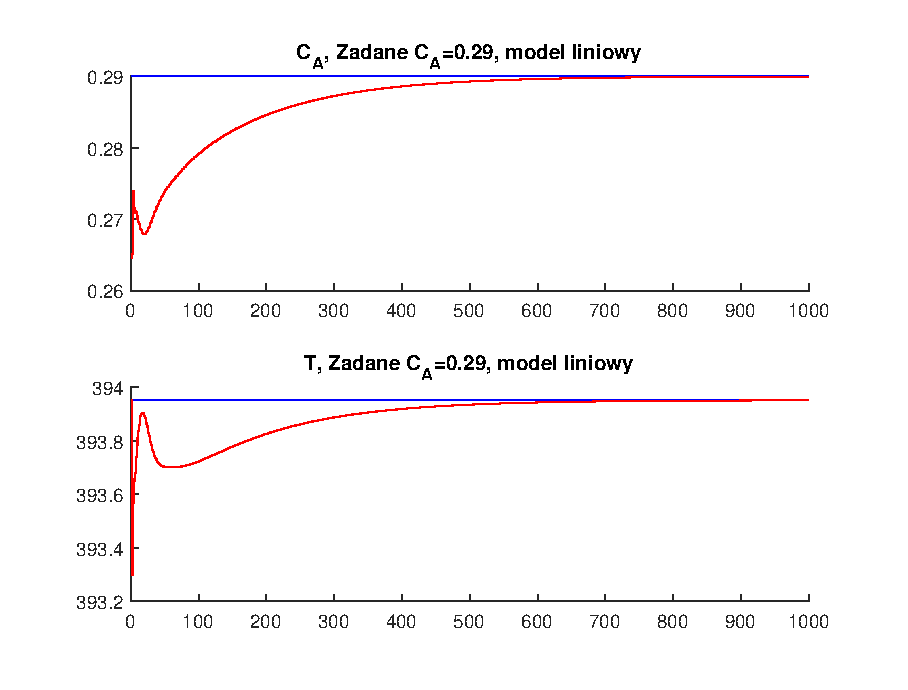
\includegraphics[width=.5\linewidth]{img/pidlin/pidlin2.eps}
		&
		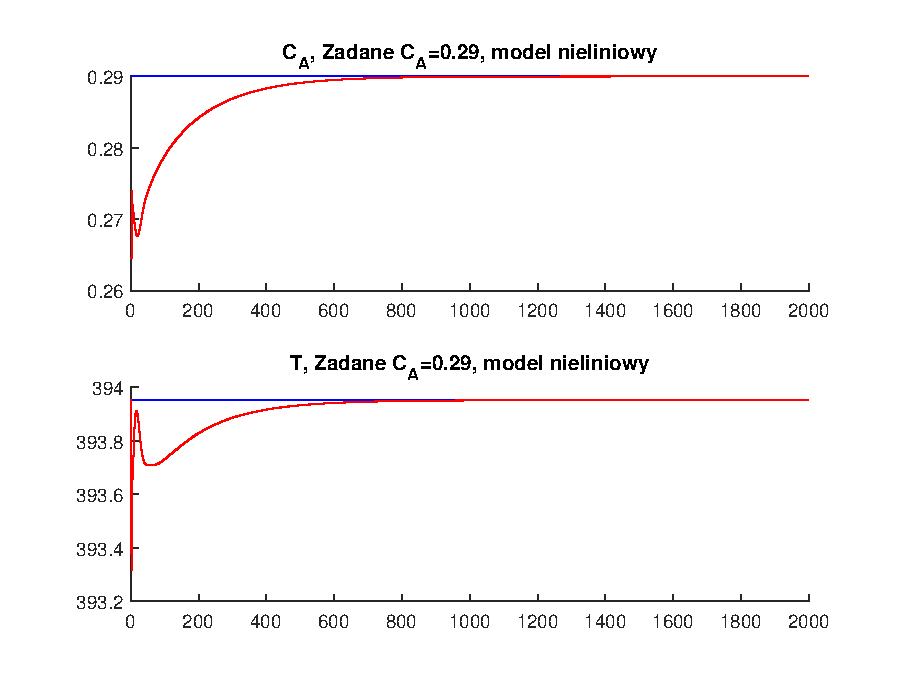
\includegraphics[width=.5\linewidth]{img/pidnlin/pidnlin2.eps}
		\\
		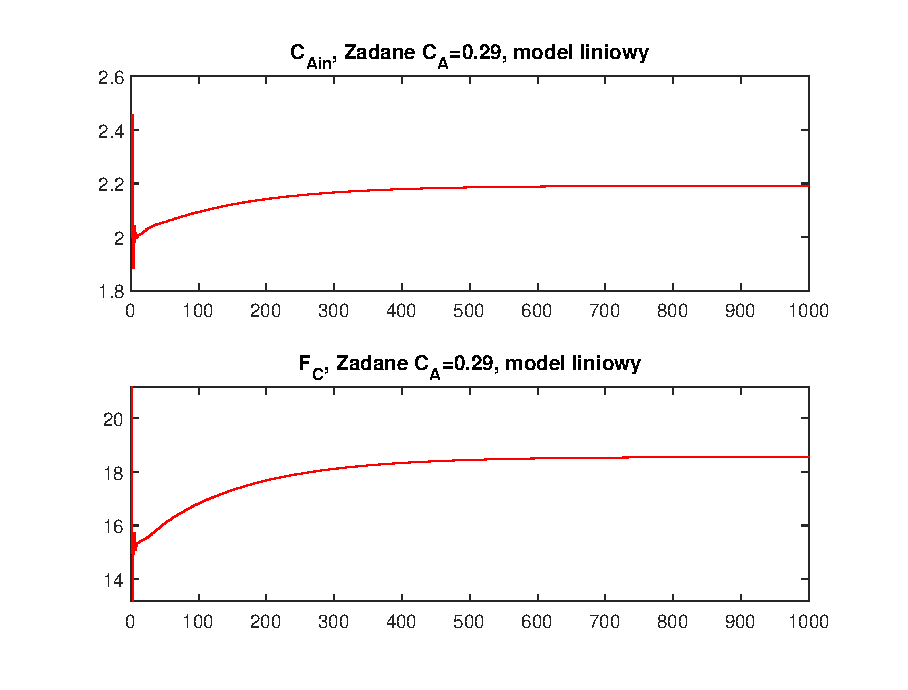
\includegraphics[width=.5\linewidth]{img/pidlin/pidlin1.eps}
		&
		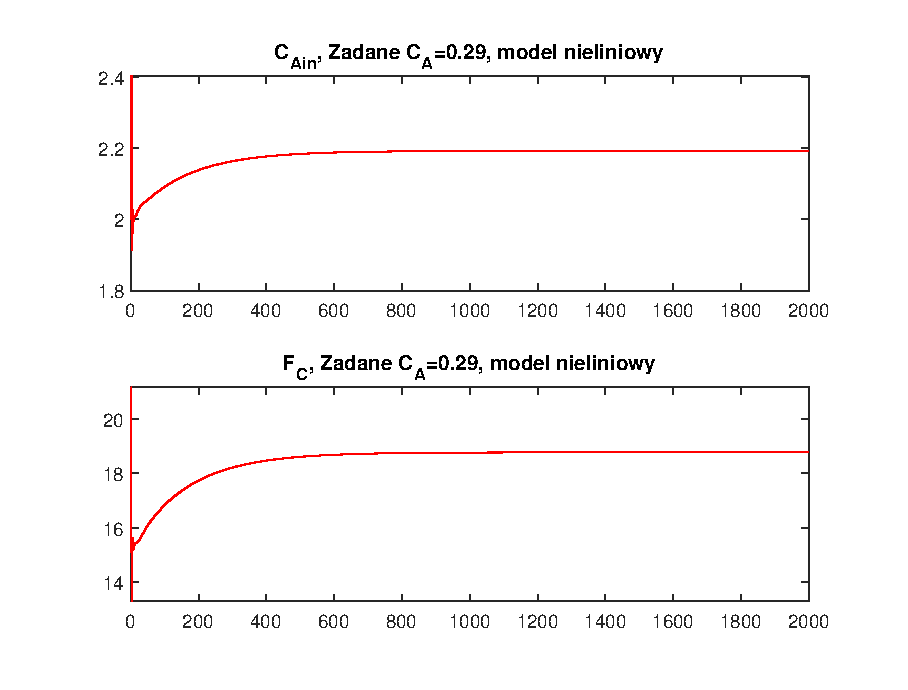
\includegraphics[width=.5\linewidth]{img/pidnlin/pidnlin1.eps}
	\end{tabular}
\label{ch2:pid1}
\caption{Regulacja PID - skok wartości zadanej $C_A$ do 0.29}
\end{figure}
\newpage
\begin{figure}
\begin{tabular}{cc}
	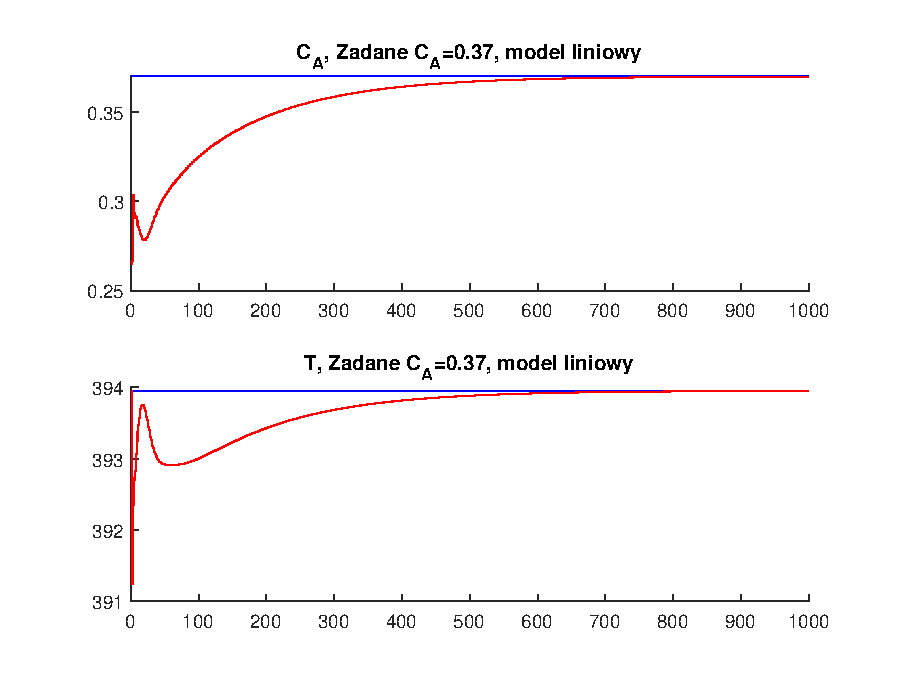
\includegraphics[width=.5\linewidth]{img/pidlin/pidlin4.eps}
	&
	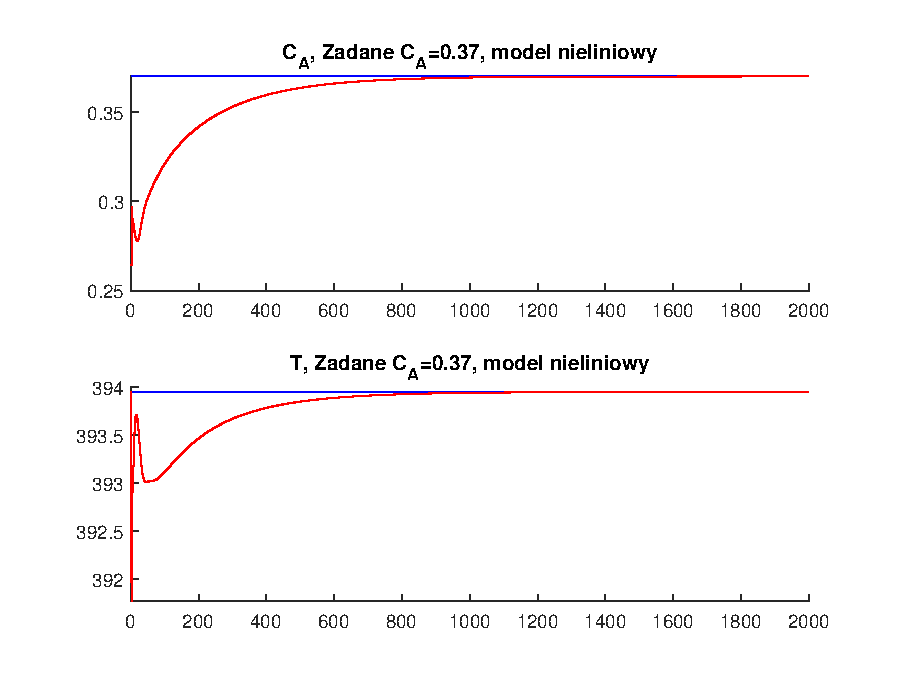
\includegraphics[width=.5\linewidth]{img/pidnlin/pidnlin4.eps}
	\\
	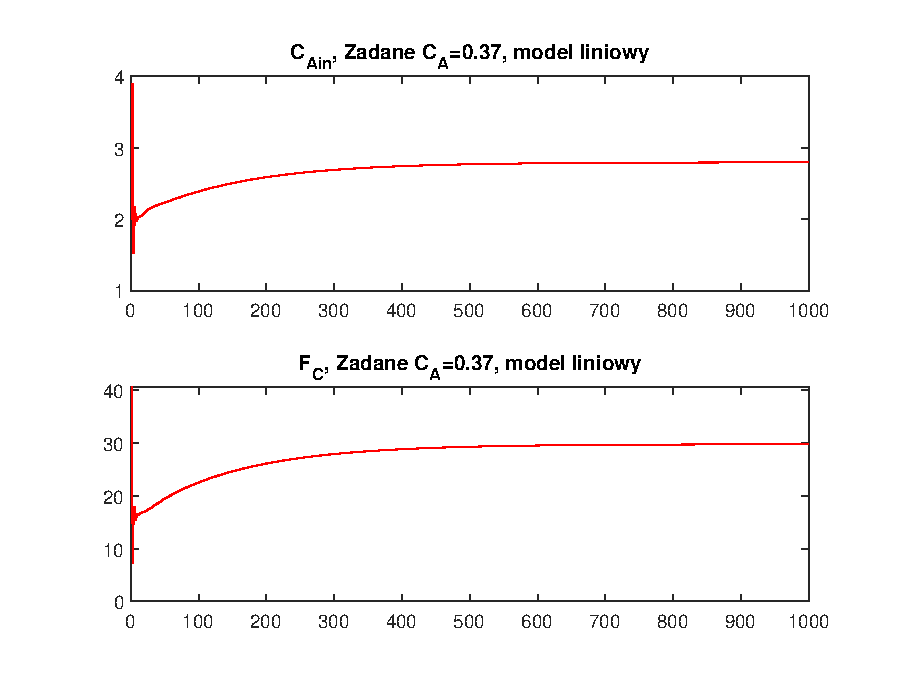
\includegraphics[width=.5\linewidth]{img/pidlin/pidlin3.eps}
	&
	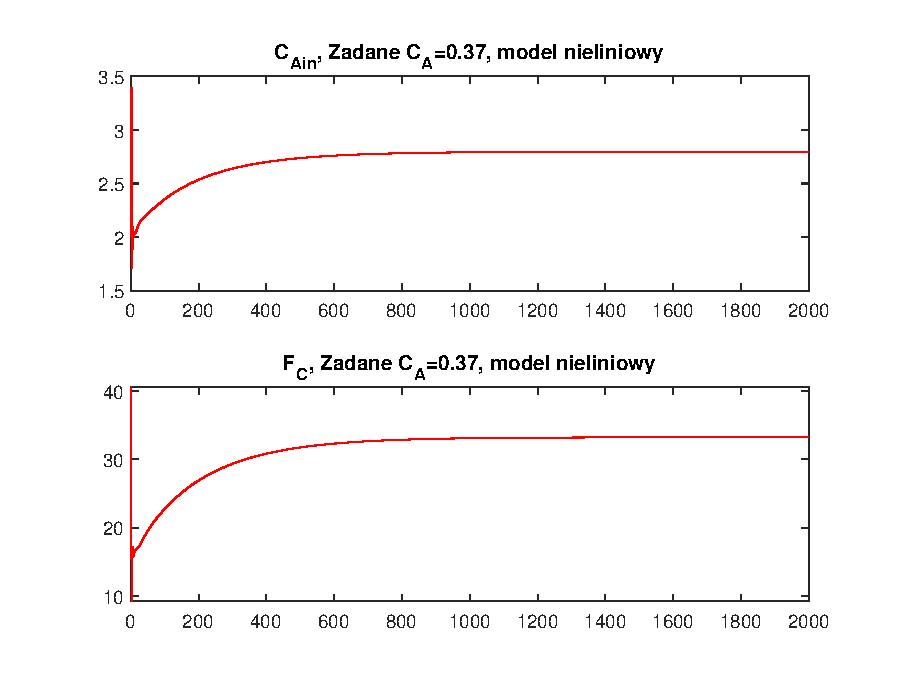
\includegraphics[width=.5\linewidth]{img/pidnlin/pidnlin3.eps}
\end{tabular}
\label{ch2:pid2}
\caption{Regulacja PID - skok wartości zadanej $C_A$ do 0.37}
\end{figure}
\newpage
\begin{figure}
\begin{tabular}{cc}
	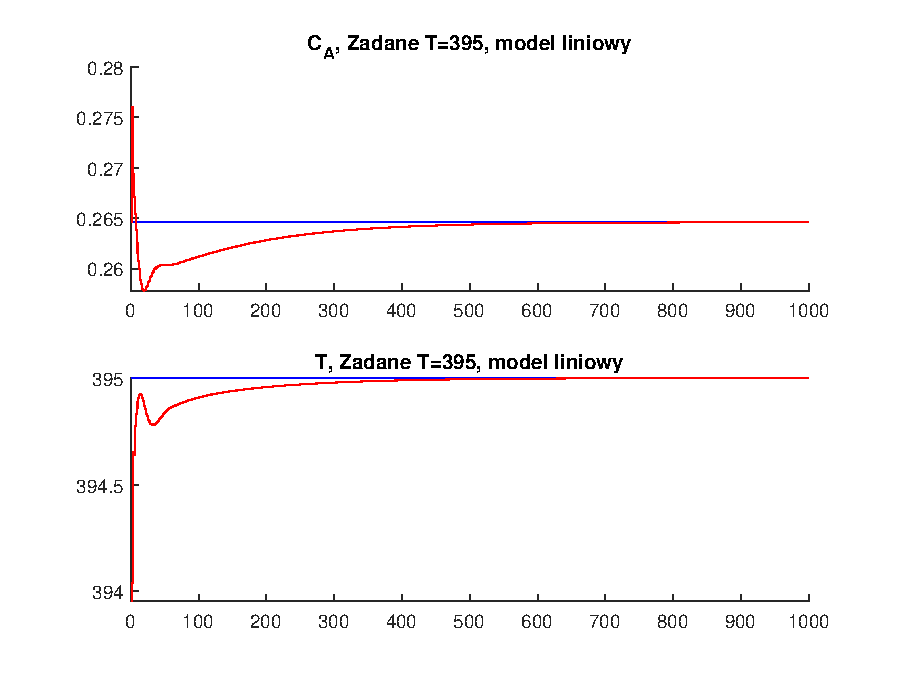
\includegraphics[width=.5\linewidth]{img/pidlin/pidlin6.eps}
	&
	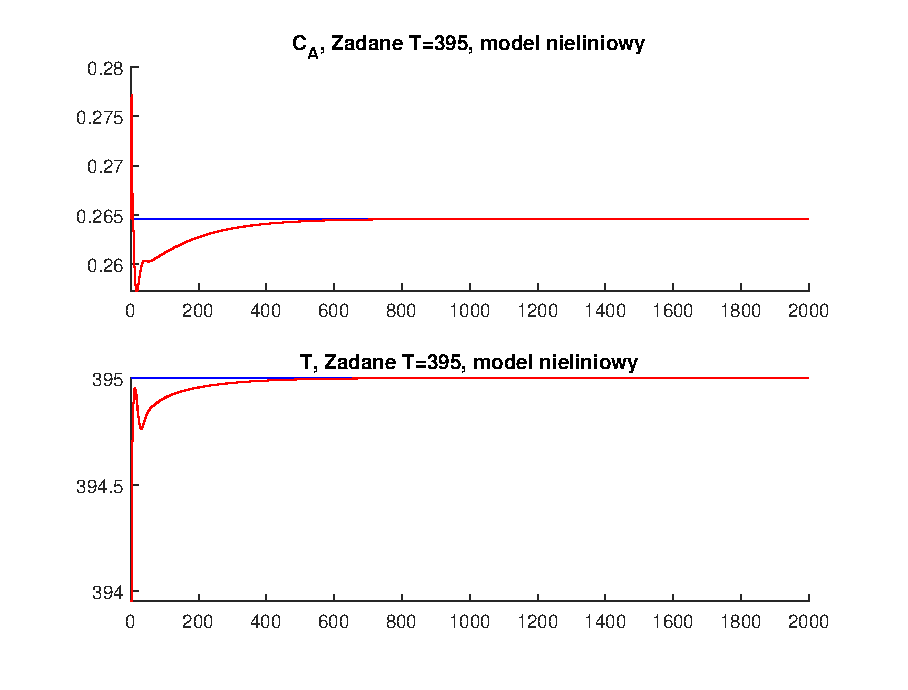
\includegraphics[width=.5\linewidth]{img/pidnlin/pidnlin6.eps}
	\\
	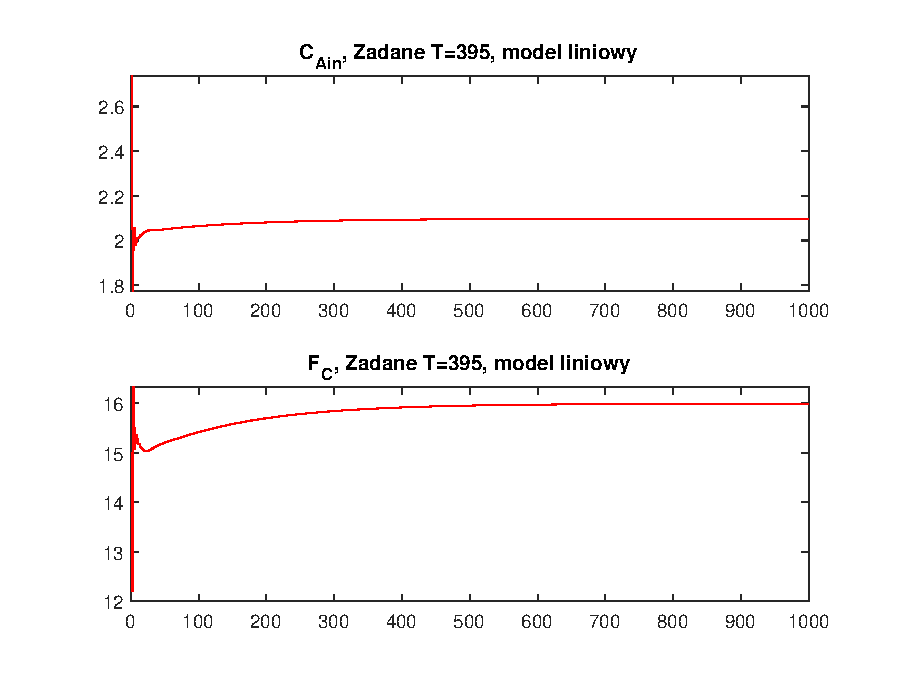
\includegraphics[width=.5\linewidth]{img/pidlin/pidlin5.eps}
	&
	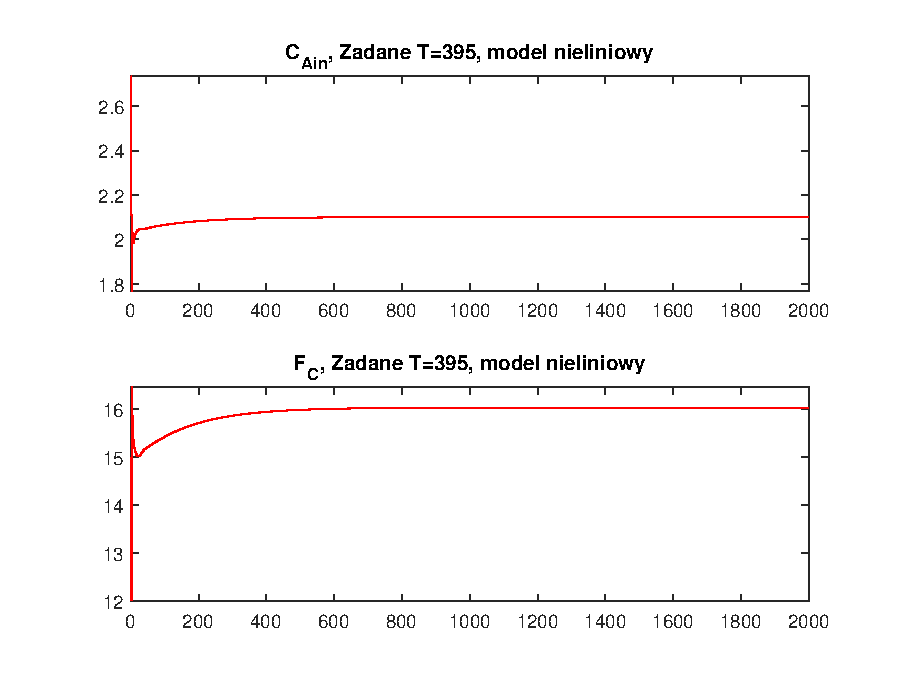
\includegraphics[width=.5\linewidth]{img/pidnlin/pidnlin5.eps}
\end{tabular}
\label{ch2:pid3}
\caption{Regulacja PID - skok wartości zadanej $T$ do 395}
\end{figure}
\newpage
\begin{figure}
\begin{tabular}{cc}
	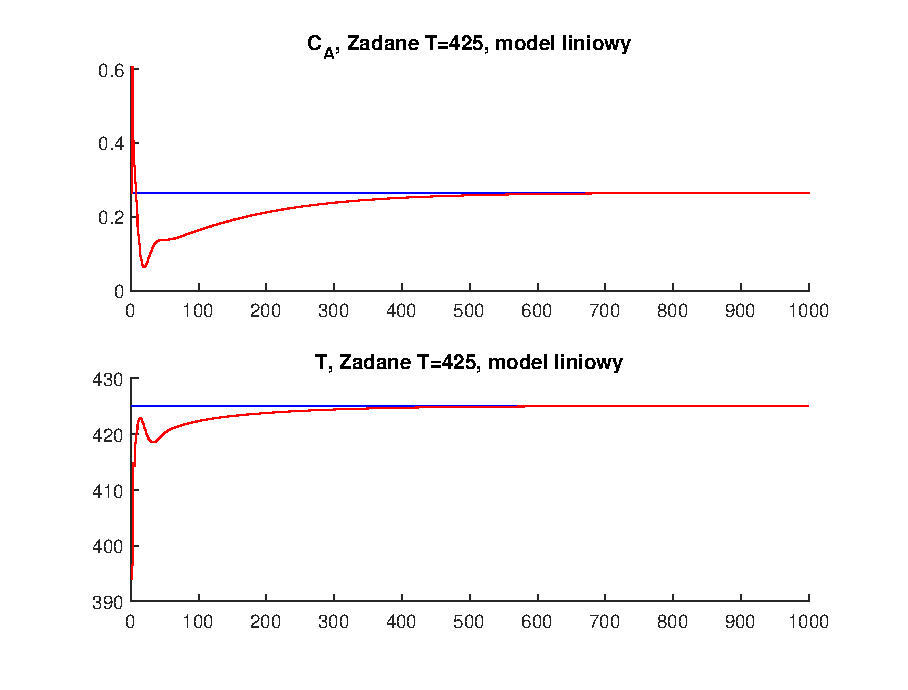
\includegraphics[width=.5\linewidth]{img/pidlin/pidlin8.eps}
	&
	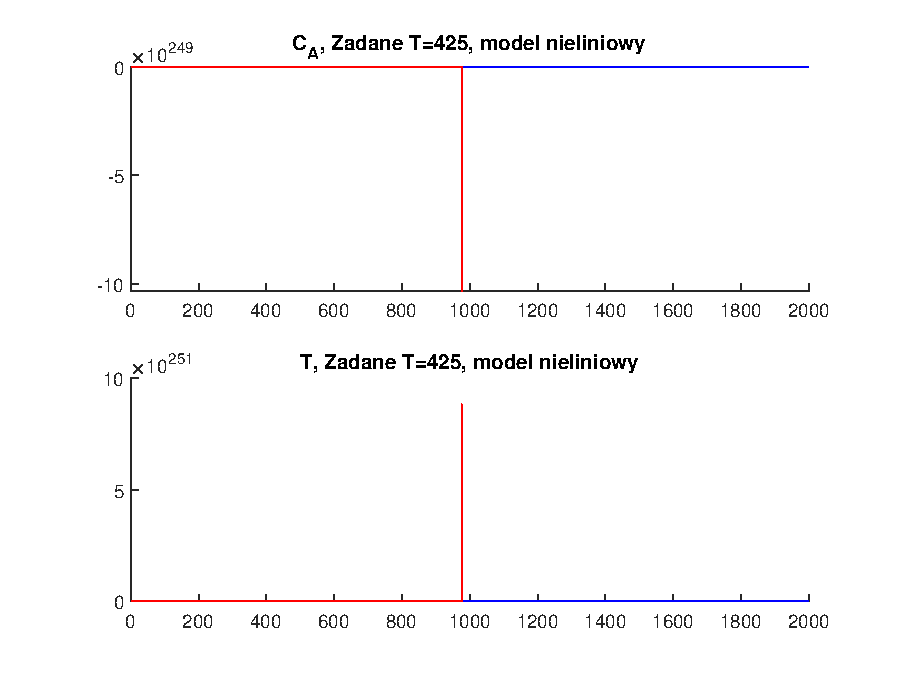
\includegraphics[width=.5\linewidth]{img/pidnlin/pidnlin8.eps}
	\\
	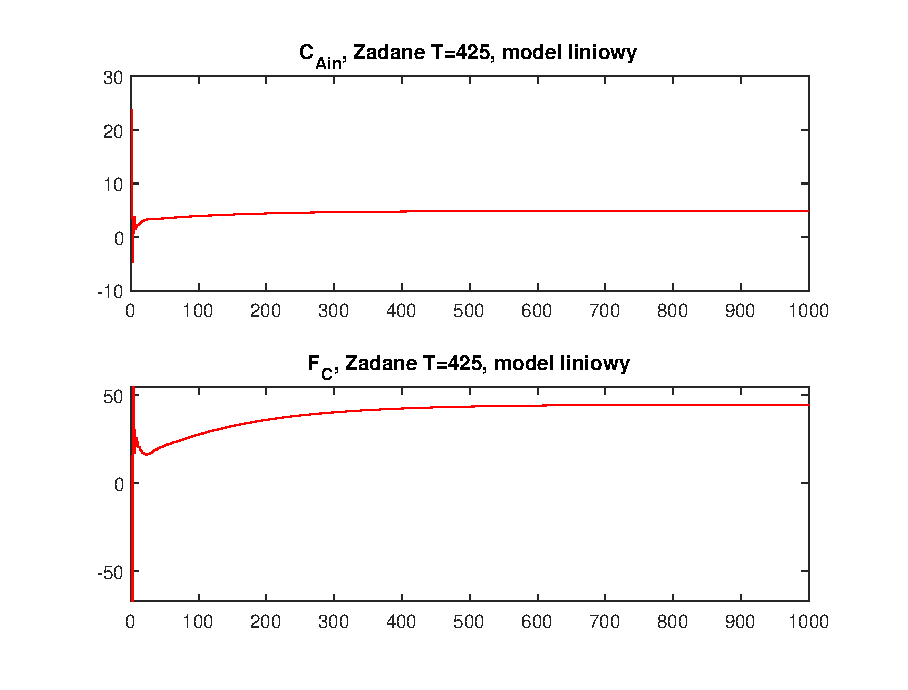
\includegraphics[width=.5\linewidth]{img/pidlin/pidlin7.eps}
	&
	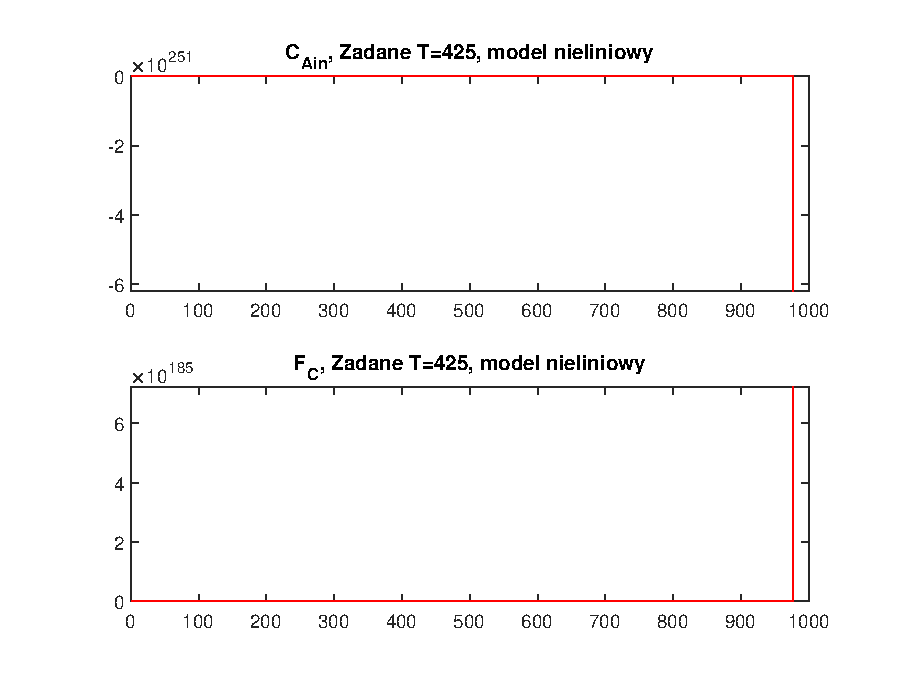
\includegraphics[width=.5\linewidth]{img/pidnlin/pidnlin7.eps}
\end{tabular}
\label{ch2:pid4}
\caption{Regulacja PID - skok wartości zadanej $T$ do 425}
\end{figure}
\newpage
\begin{figure}
\begin{tabular}{cc}
	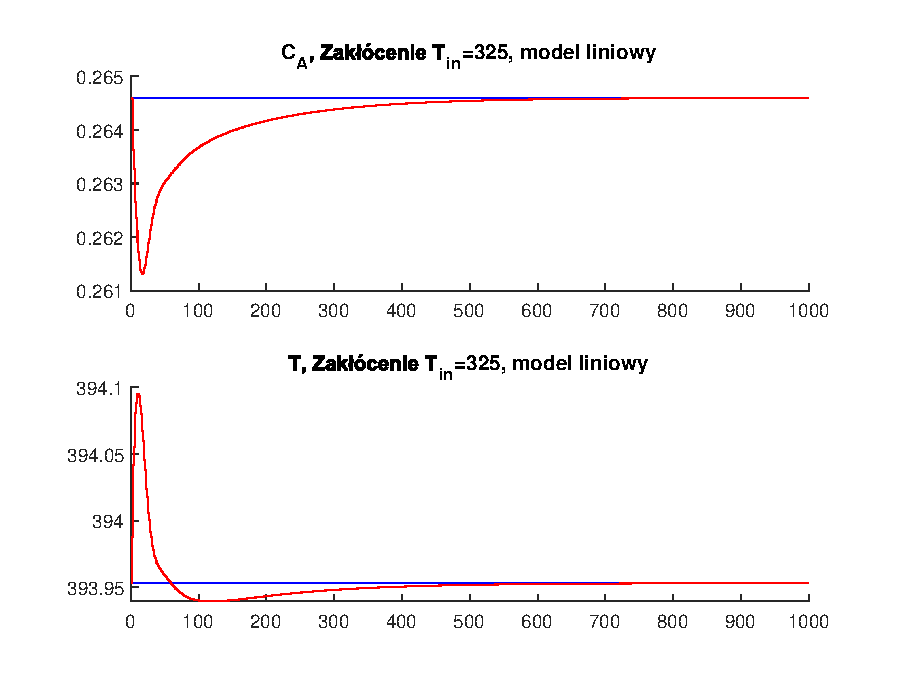
\includegraphics[width=.5\linewidth]{img/pidlin/pidlin10.eps}
	&
	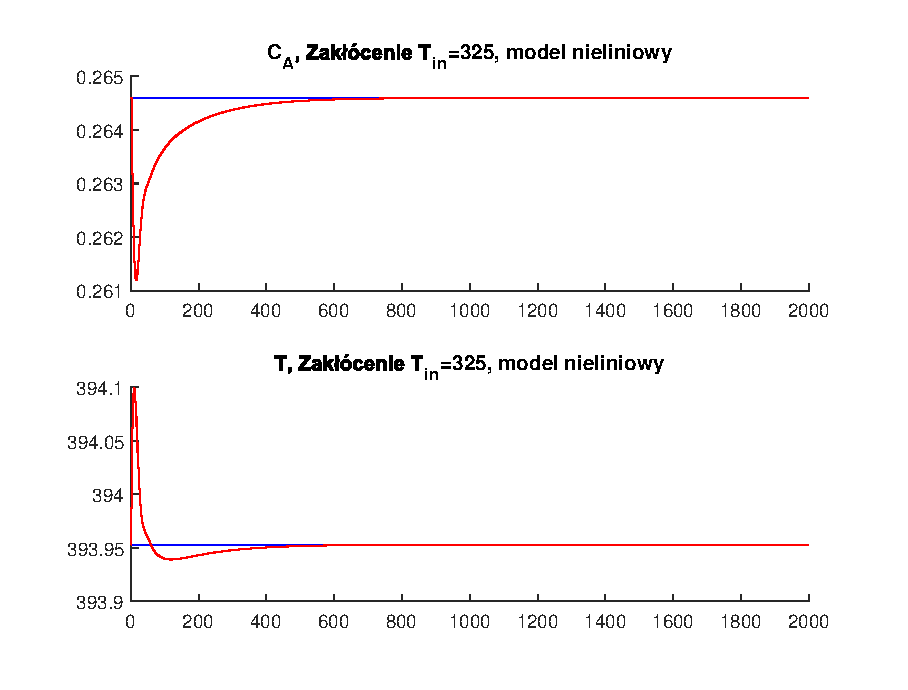
\includegraphics[width=.5\linewidth]{img/pidnlin/pidnlin10.eps}
	\\
	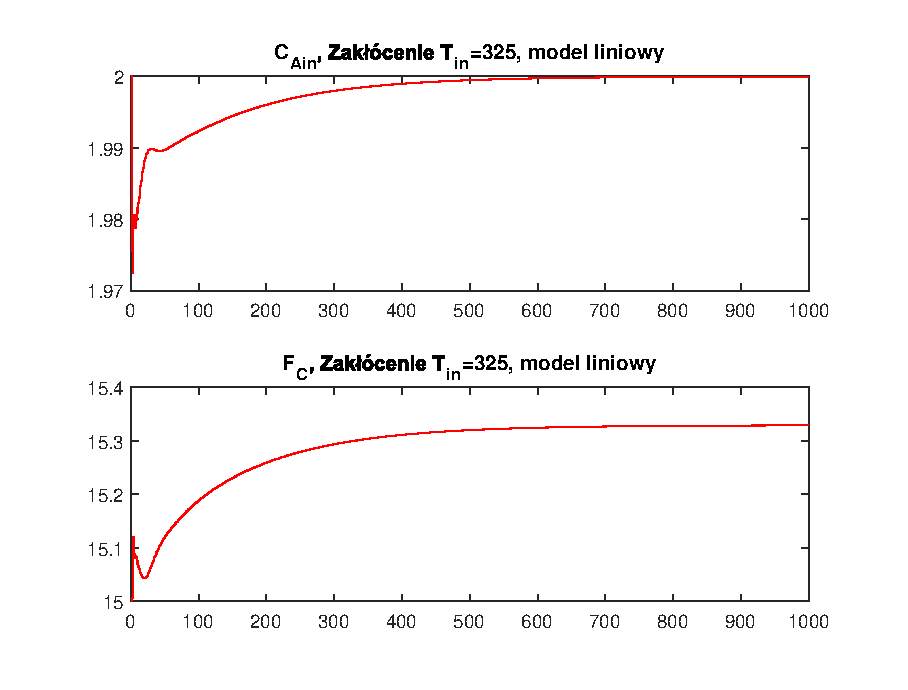
\includegraphics[width=.5\linewidth]{img/pidlin/pidlin9.eps}
	&
	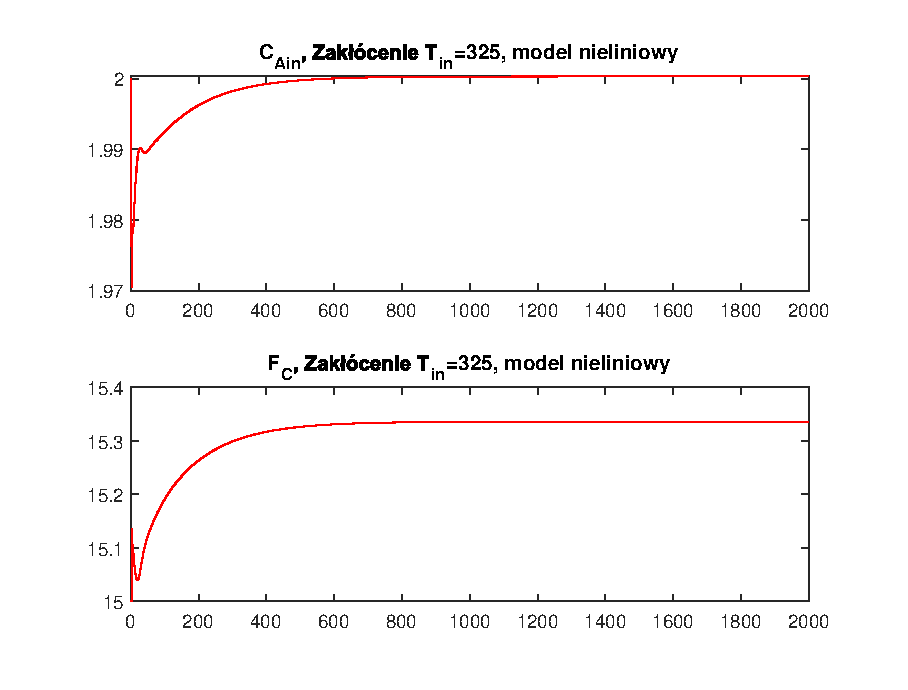
\includegraphics[width=.5\linewidth]{img/pidnlin/pidnlin9.eps}
\end{tabular}
\label{ch2:pid5}
\caption{Regulacja PID - skok zakłócenia $T_{in}$ do 325}
\end{figure}
\newpage
\begin{figure}
\begin{tabular}{cc}
	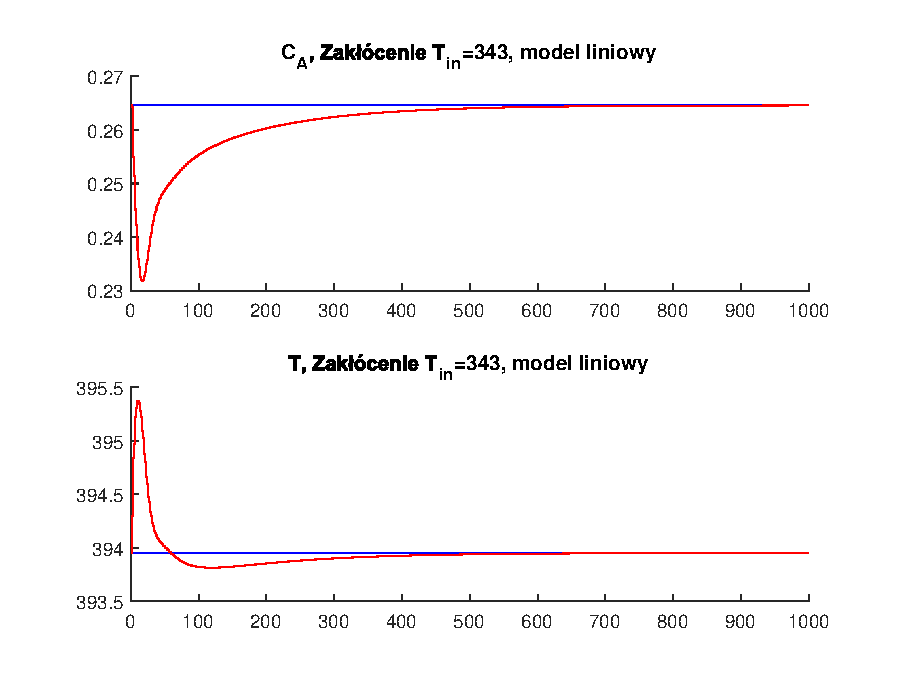
\includegraphics[width=.5\linewidth]{img/pidlin/pidlin12.eps}
	&
	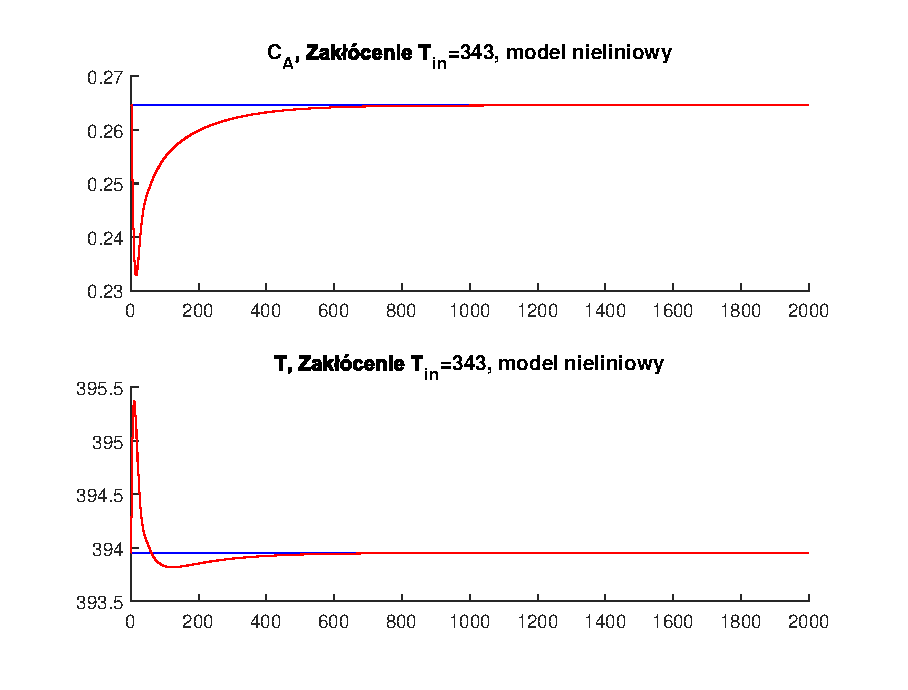
\includegraphics[width=.5\linewidth]{img/pidnlin/pidnlin12.eps}
	\\
	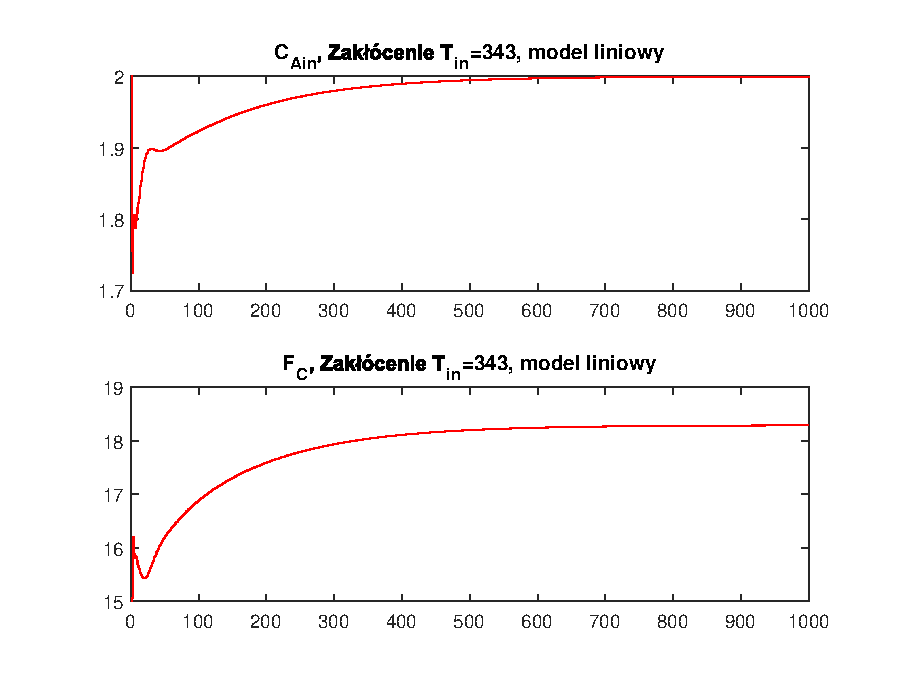
\includegraphics[width=.5\linewidth]{img/pidlin/pidlin11.eps}
	&
	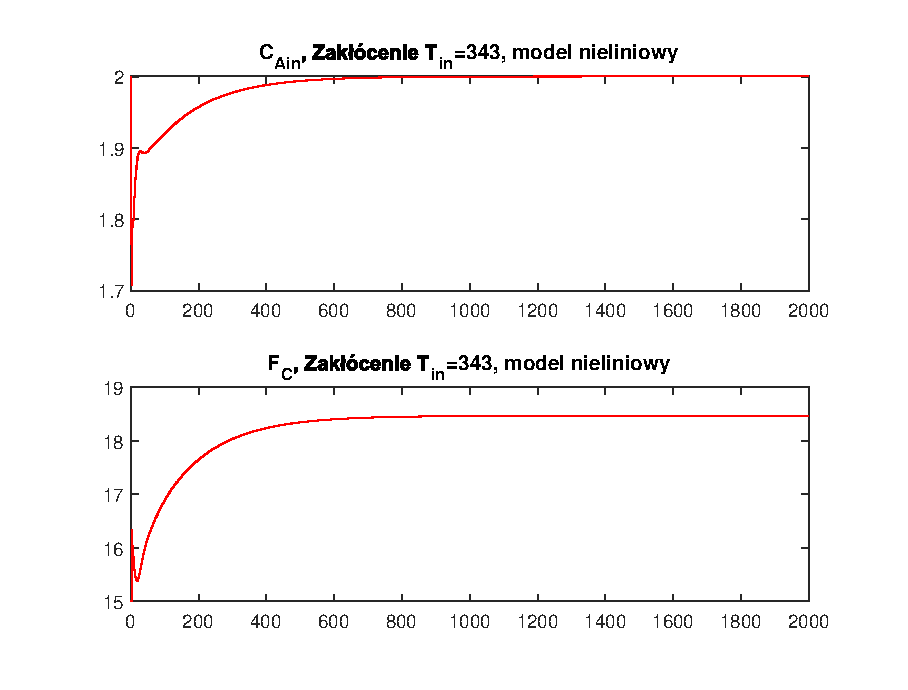
\includegraphics[width=.5\linewidth]{img/pidnlin/pidnlin11.eps}
\end{tabular}
\label{ch2:pid6}
\caption{Regulacja PID - skok zakłócenia $T_{in}$ do 343}
\end{figure}
\newpage
\begin{figure}
\begin{tabular}{cc}
	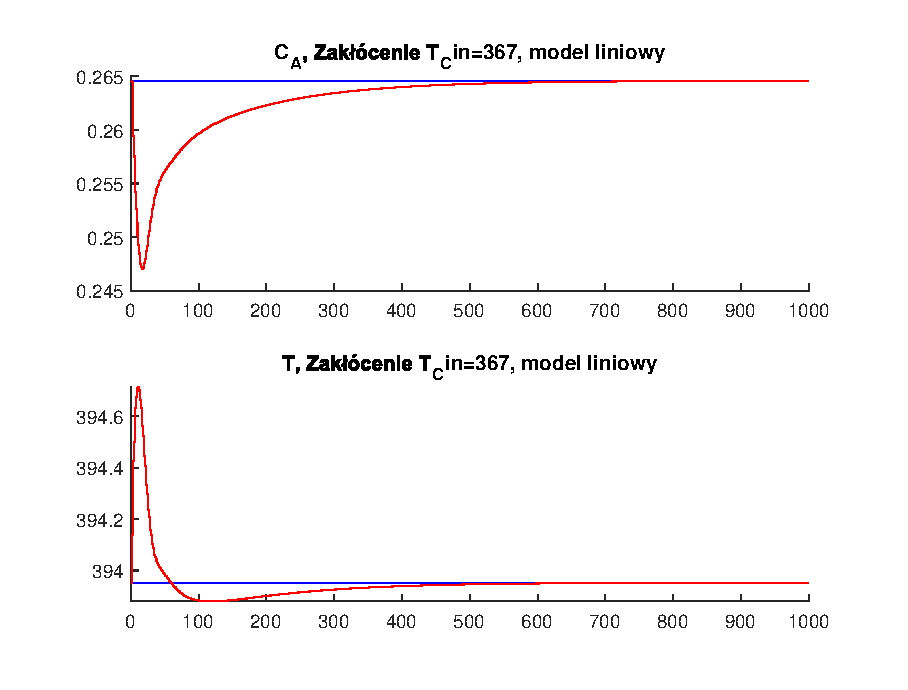
\includegraphics[width=.5\linewidth]{img/pidlin/pidlin14.eps}
	&
	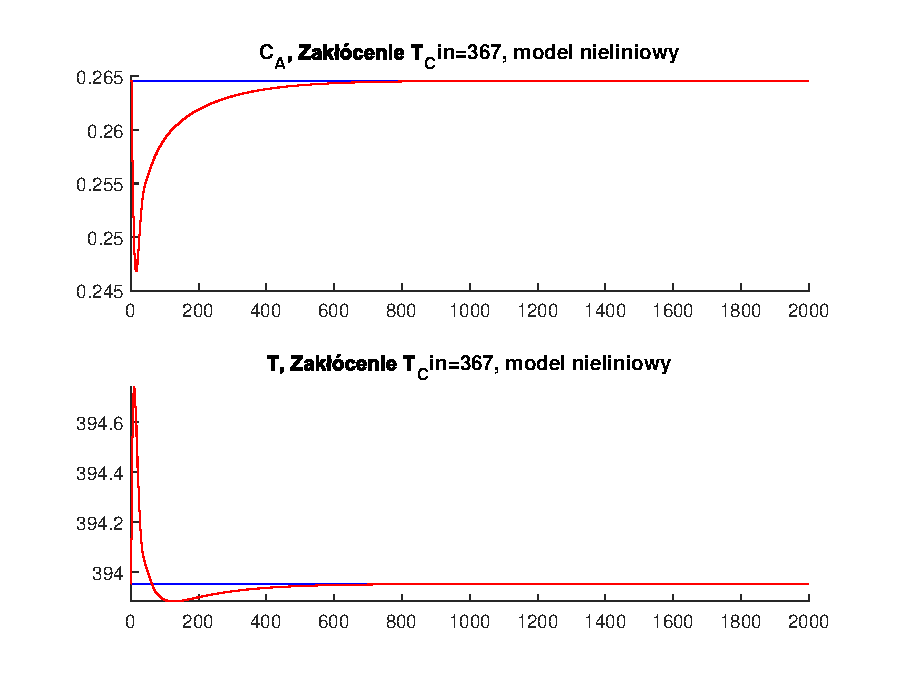
\includegraphics[width=.5\linewidth]{img/pidnlin/pidnlin14.eps}
	\\
	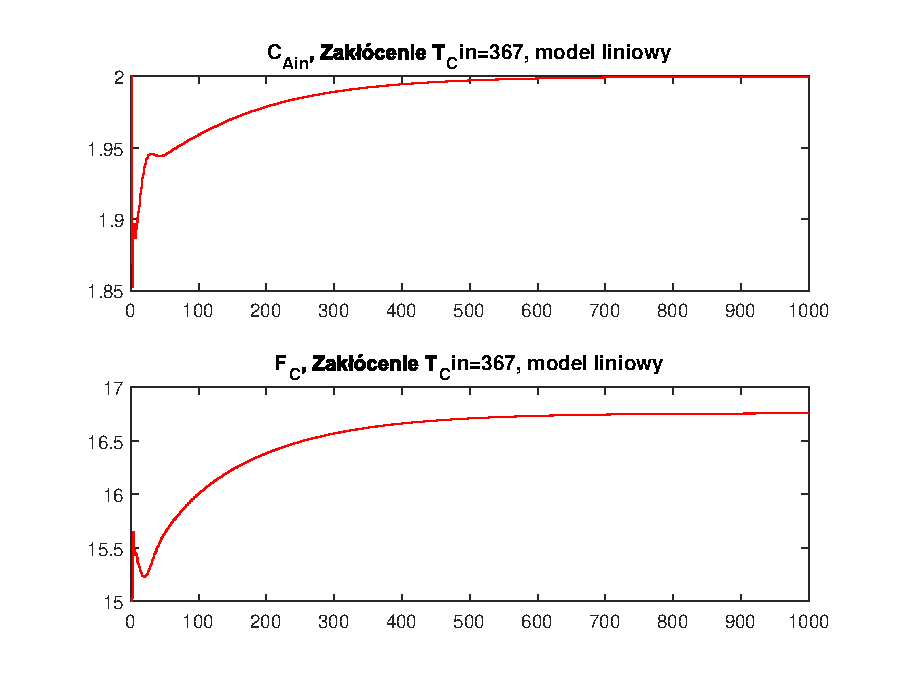
\includegraphics[width=.5\linewidth]{img/pidlin/pidlin13.eps}
	&
	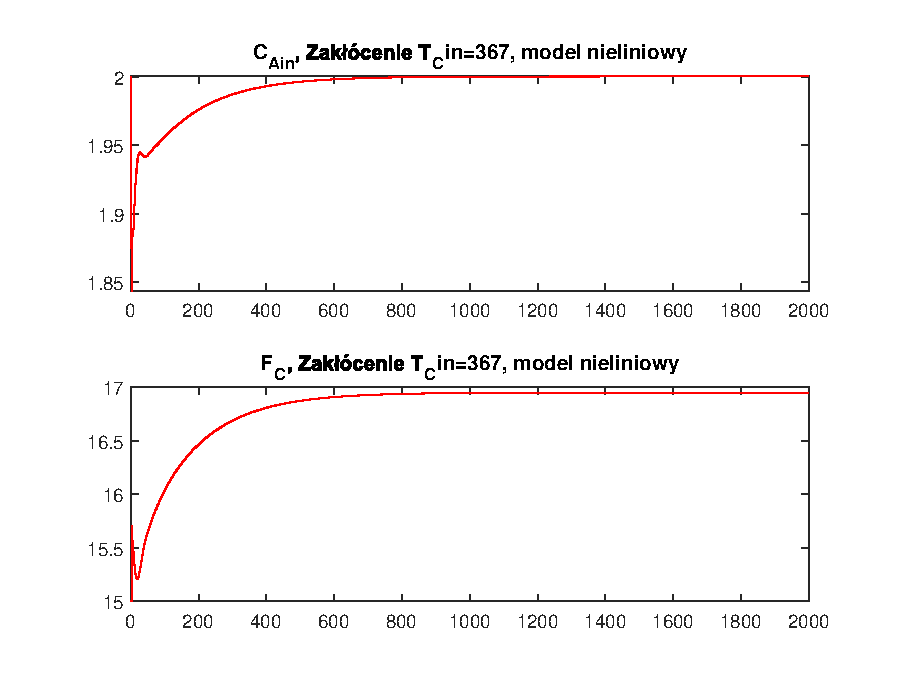
\includegraphics[width=.5\linewidth]{img/pidnlin/pidnlin13.eps}
\end{tabular}
\label{ch2:pid7}
\caption{Regulacja PID - skok zakłócenia $T_{Cin}$ do 367}
\end{figure}
\newpage
\begin{figure}
\begin{tabular}{cc}
	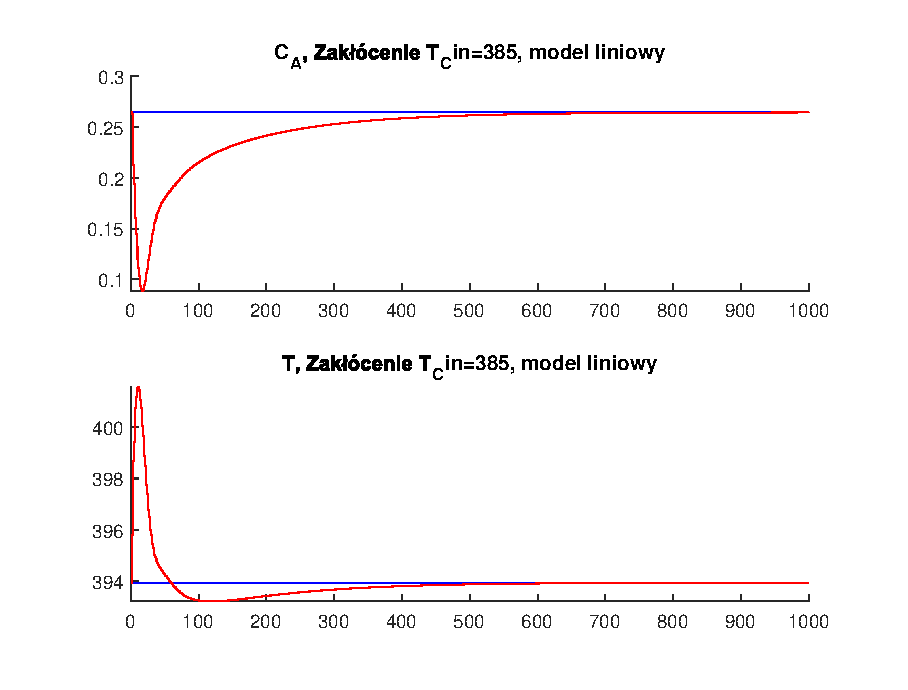
\includegraphics[width=.5\linewidth]{img/pidlin/pidlin16.eps}
	&
	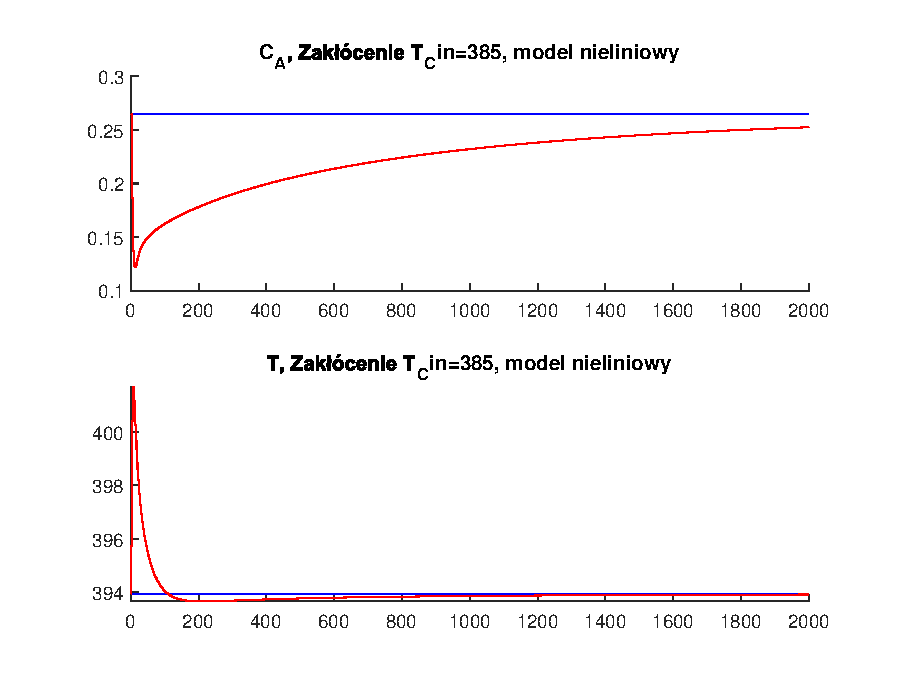
\includegraphics[width=.5\linewidth]{img/pidnlin/pidnlin16.eps}
	\\
	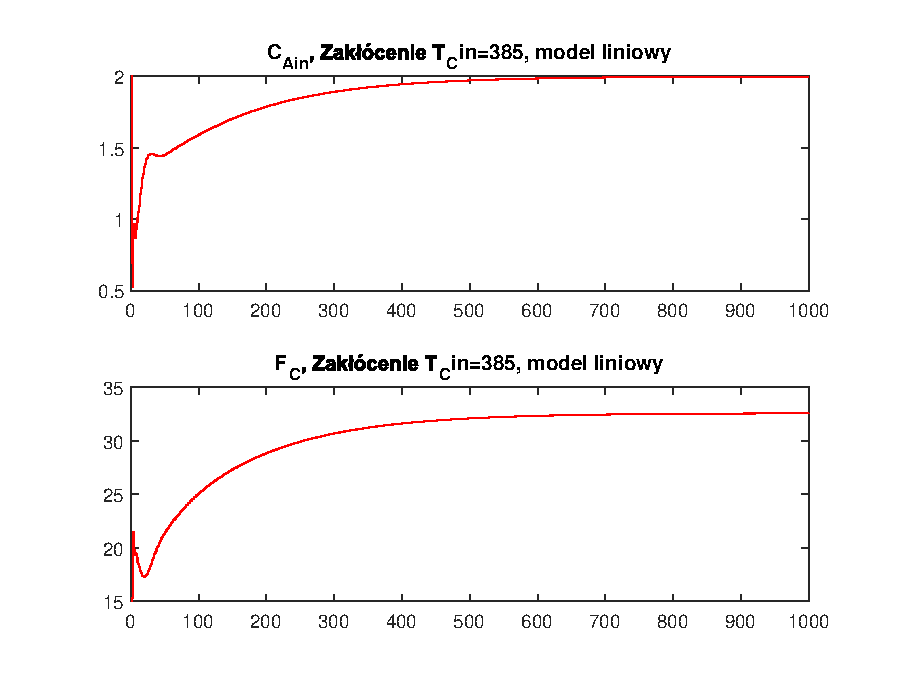
\includegraphics[width=.5\linewidth]{img/pidlin/pidlin15.eps}
	&
	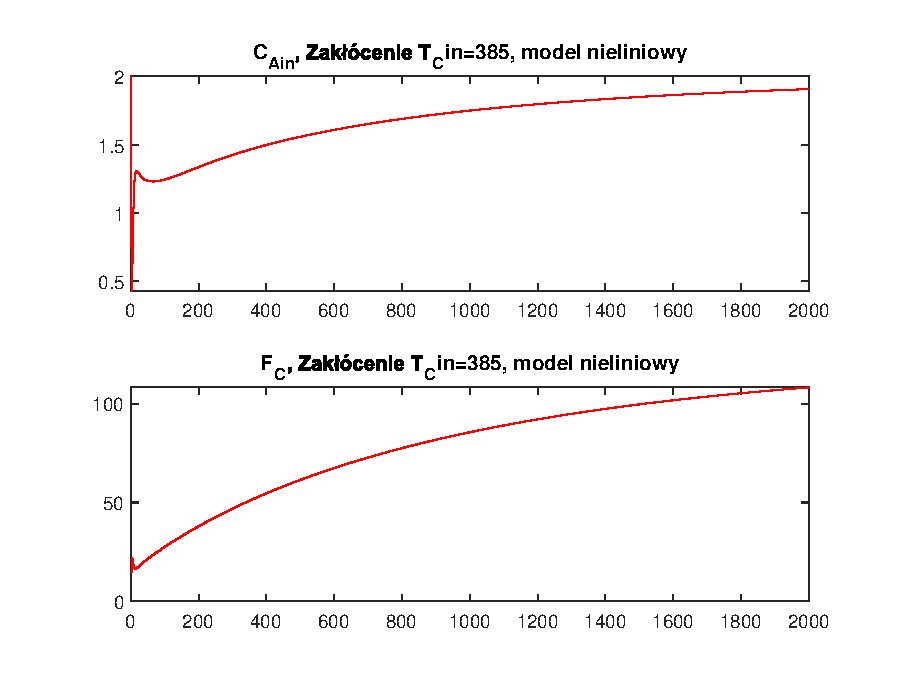
\includegraphics[width=.5\linewidth]{img/pidnlin/pidnlin15.eps}
\end{tabular}
\label{ch2:pid8}
\caption{Regulacja PID - skok zakłócenia $T_{Cin}$ do 385}
\end{figure}

\section{Regulacja DMC}
\begin{figure}[h!]
	\centering
	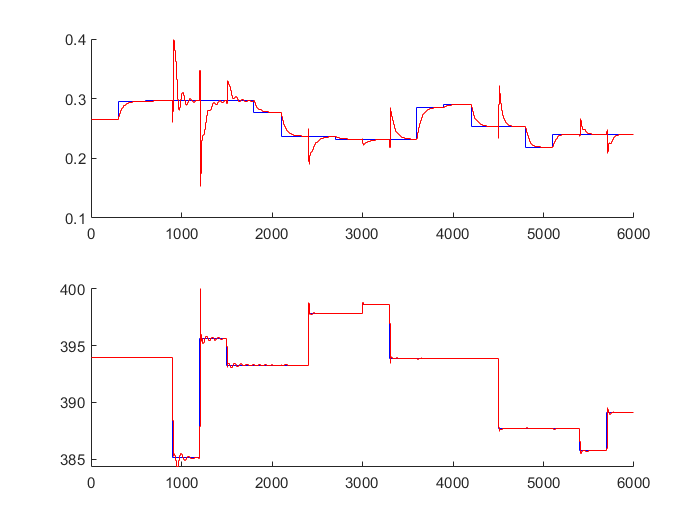
\includegraphics[width=.6\linewidth]{img/yDMC.png}
	\label{ch2:Zadanie}
	\caption{Regulacja DMC analityczna - wyjście na tle wartości zadanej}
\end{figure}
\begin{figure}[h!]
	\centering
	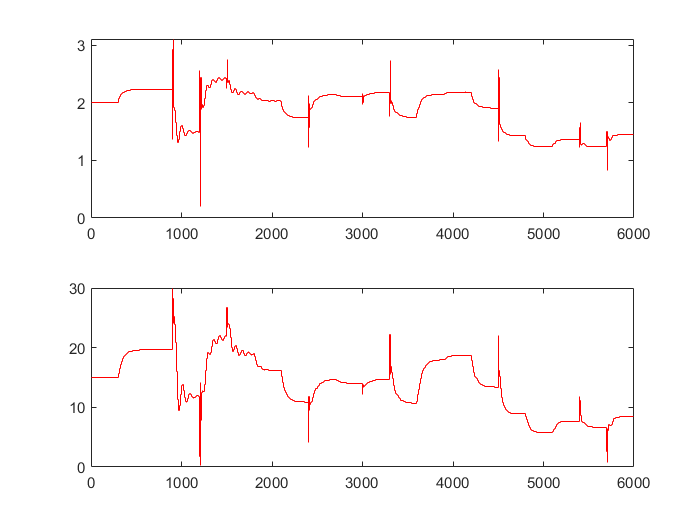
\includegraphics[width=.6\linewidth]{img/uDMC.png}
	\label{ch2:Zadanie}
	\caption{Regulacja DMC analityczna - sterowanie}
\end{figure}
\begin{figure}[h!]
	\centering
	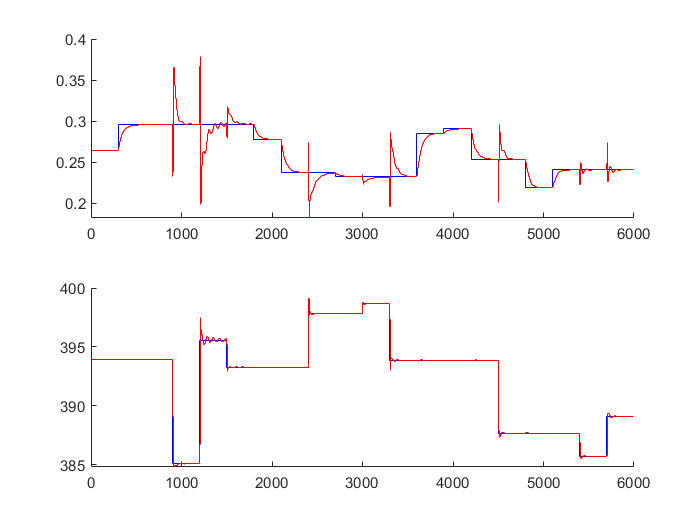
\includegraphics[width=.6\linewidth]{img/yDMCnum.png}
	\label{ch2:Zadanie}
	\caption{Regulacja DMC numeryczna - wyjście na tle wartości zadanej}
\end{figure}
\begin{figure}[h!]
	\centering
	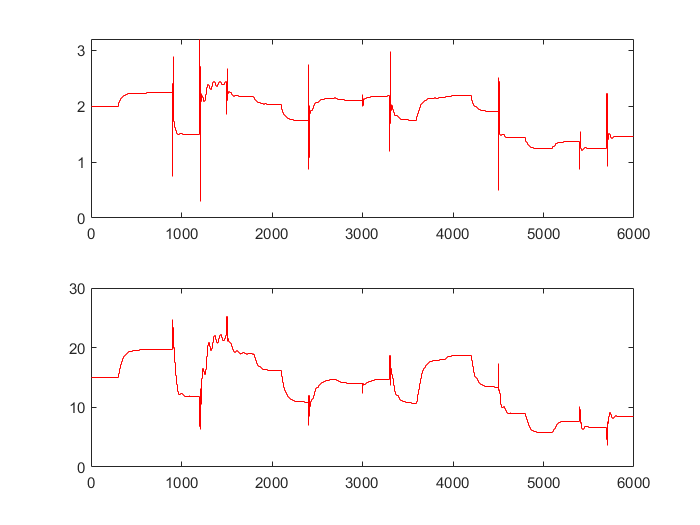
\includegraphics[width=.6\linewidth]{img/uDMCnum.png}
	\label{ch2:Zadanie}
	\caption{Regulacja DMC numeryczna - sterowanie}
\end{figure}
\newpage
Działanie prezentowanych powyżej algorytmów najłatwiej porównać będzie prezentując je na wspólnym rysunku. 
Zgodnie z oczekiwaniami, regulacja przebieg w podobny sposób dla obu implementacji regulatora. W obu przypadkach występują oscylacje wyjścia przy dużych skokach wartości zadanej dla wyjścia T procesu, dla niewielkich skoków wartości zadanej, regulatory porównywalnie szybko sprowadzają wartość wyjścia T do zadanego poziomu. Wyjście CA również zachowuje porównywaly przebied przy zastosowaniu regulatora analitycznego, czy numerycznego. Ta zmienna wyjściowa, nieco wrażliwsza w regulacji, a oba typy regulatorów spowodowały zbliżony, a często pokrywający się przebieg, z podobnymi wysokościami przeregulowań.
Należy jednak zaznaczyć, że mimo podobieństwa wyników i przebiegu sterowań, obliczenia dla algorytmu numerycznego trwały znacznie dłużej niż dla analitycznego.
\begin{figure}[h!]
	\centering
	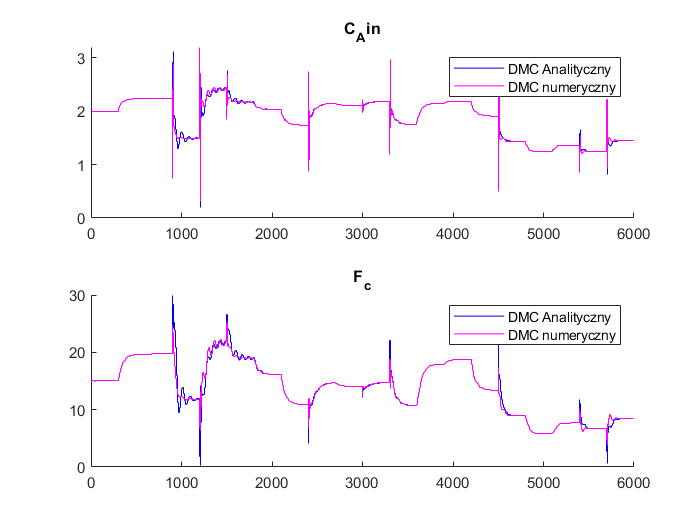
\includegraphics[width=.6\linewidth]{img/uComparedDMC.png}
	\label{ch2:Zadanie}
	\caption{Regulacja DMC analityczna i numeryczna - sterowanie}
\end{figure}
\begin{figure}[h!]
	\centering
	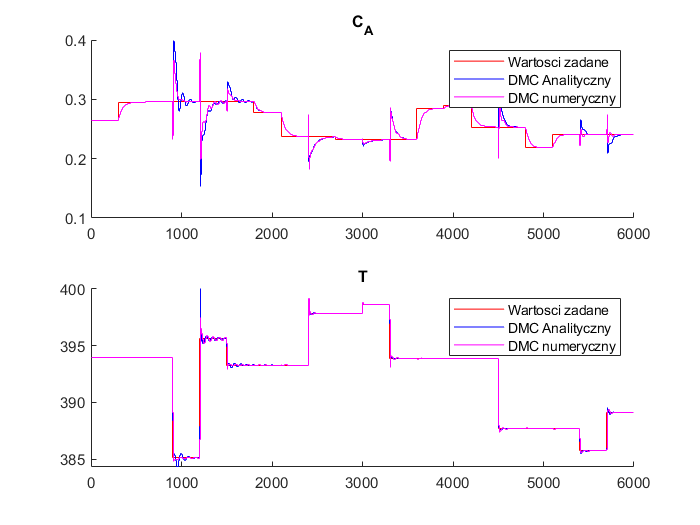
\includegraphics[width=.6\linewidth]{img/yComparedDMC.png}
	\label{ch2:Zadanie}
	\caption{Regulacja DMC analityczna i numeryczna - wyjścia}
\end{figure}